\documentclass[tikz,border=8pt]{standalone}
\usepackage{amsmath,amssymb}
\usepackage{tikz}
\usepackage{pgfplots}
\pgfplotsset{compat=1.18}
\begin{document}
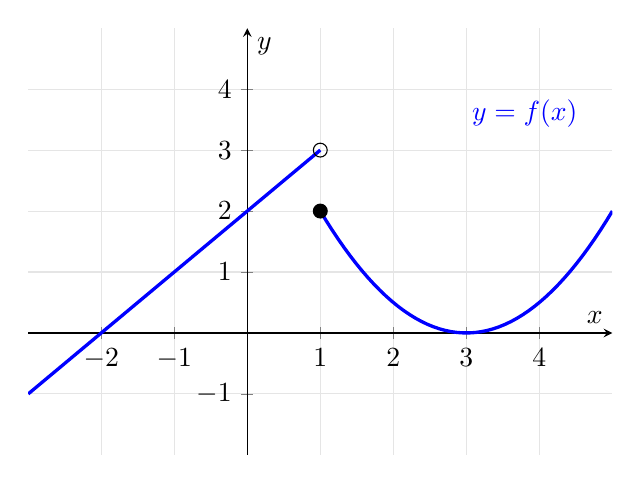
\begin{tikzpicture}
  \begin{axis}[
    axis lines=middle, xlabel={$x$}, ylabel={$y$},
    xmin=-3, xmax=5, ymin=-2, ymax=5,
    xtick={-2,...,4}, ytick={-1,...,4},
    grid=both, grid style={gray!20},
    width=9cm, height=7cm,
  ]
    \addplot[very thick, blue, domain=-3:1] {x + 2};
    \addplot[very thick, blue, domain=1:5, samples=50] {(x-3)^2/2};
    % x=1 noktasında soldan limit 3, f(1)=2 (dolu), sağdan limit 2
    \addplot[only marks, mark=o, mark size=2.5pt, fill=white] coordinates {(1,3)};
    \addplot[only marks, mark=*, mark size=2.5pt] coordinates {(1,2)};
    \node[blue] at (axis cs:3.8,3.6) {$y=f(x)$};
  \end{axis}
\end{tikzpicture}
\end{document}
